\section{Durchführung}
\label{sec:Durchführung}

Dieser Versuch wurde nicht real durchgeführt, es wurden nur entsprechende Messreihen zur Verfügung gestellt,
sodas hier nur eine theoretische Durchführung beschrieben werden kann. Dazu sei hier zunächst der schematische Aufbau 
der Wärmepumpe dargestellt:\ref{fig:Abb1} 

\begin{figure}
    \centering
    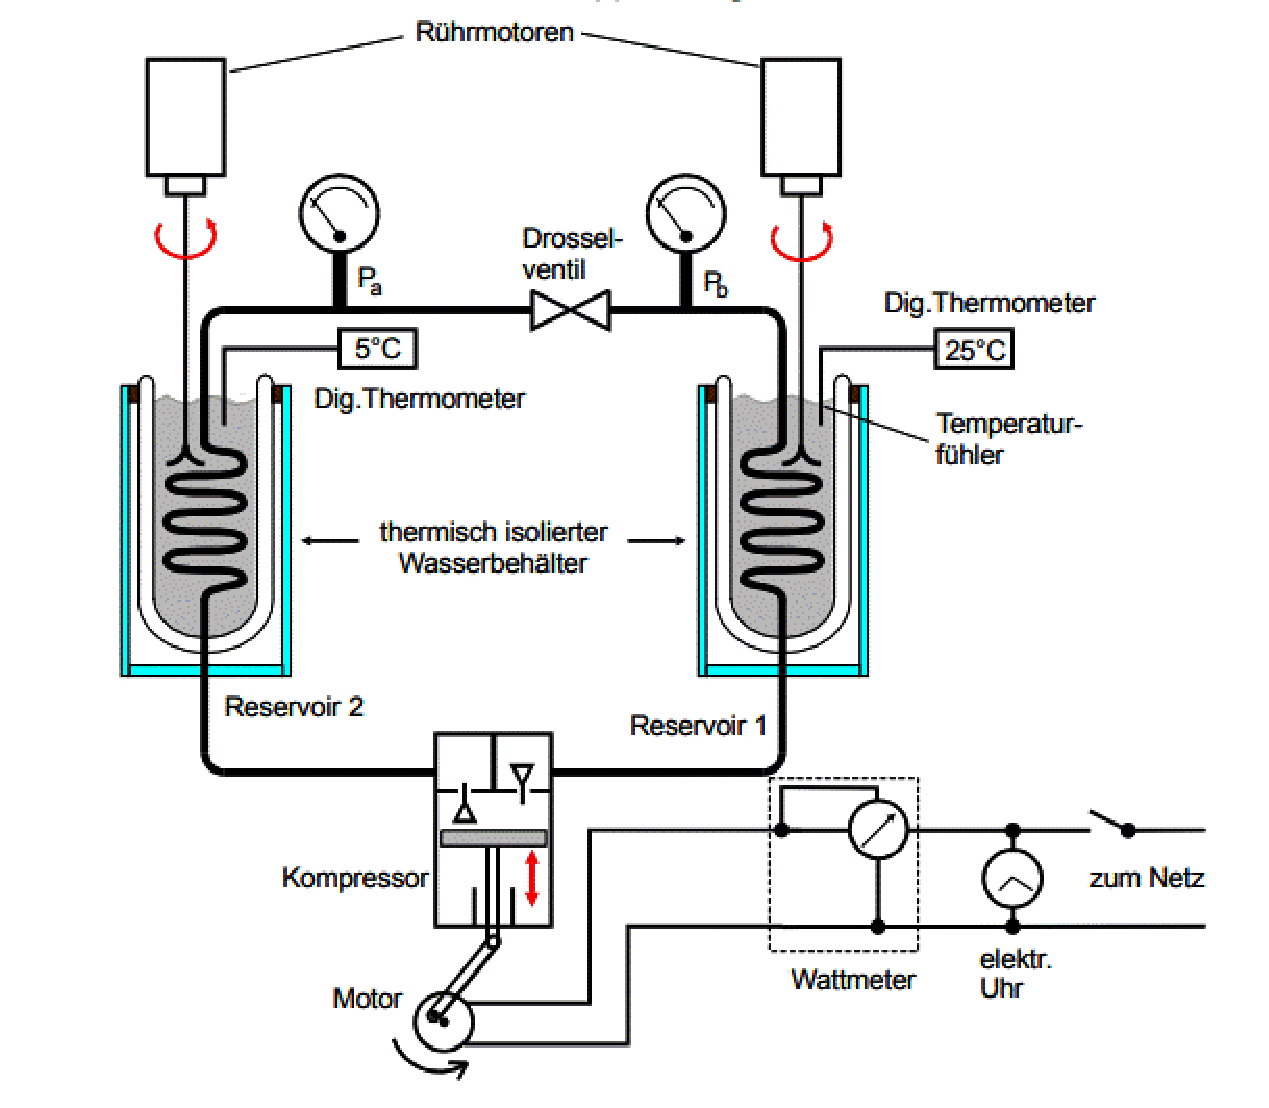
\includegraphics[width=15cm,height=13cm]{SchemaWarmepumpe.pdf}
    \caption{Schematischer Aufbau der Wärmepumpe.}
    \label{fig:Abb.1}
  \end{figure}

\noindent Die Abbildung \ref{fig:Abb1} zeigt den Schematischen Aufbau der Wärmepumpe. Es gibt zwei wassergefüllte
Reservoire, das Wasser wird durch jewils einen Rührmotor in Bewegung gehalten. Durch das Wasser 
in den Reservoiren verläuft ein mehrfach gewundenes Rohr. Die Rohre sind oben über ein Drosselventil 
miteinander verbunden, jeweils vor und hinter dem Drosselventil wird mit einem Manometer der Druck gemessen.
Unten sind die Rohrwindungen über einen Kompressor verbunden. Im weiteren sind Messgeräte für die 
Wassertemperaturen in den Reservoiren(Thermometer), die Leistung elektrische Leistung des 
Kompressors (Wattmeter) und die Zeit (Uhr) vorhanden. \\


\noindent Zunächst wird die Messapparatur mit einer genau bestimmten Wassemenge befüllt. Anschließend werden die Rührmotoren
und der Kompressor eingeschaltet. Sobald das geschehen ist werden im Minutentakt
die Drücke ~$p_a$ ~ und ~$p_b$ 
sowie die Temperaturen ~$T_1 $
und ~$T_2$ wie auch die Leistungsaufnahme des Kompressors abgelesen und notiert. 
